\documentclass{article}
\usepackage{polski}
\usepackage[utf8]{inputenc}
\usepackage{float}
\usepackage{graphicx}
\usepackage{caption}
\usepackage{subcaption}
\usepackage{ragged2e}
\usepackage{amsmath}
\usepackage{amssymb}
\usepackage{amsfonts}
\usepackage{blindtext}
\usepackage{hyperref}
\usepackage{algorithmicx}
\usepackage{algpseudocode}
\usepackage{listings}
\usepackage{booktabs}
\usepackage{siunitx}
\usepackage{multicol}
\usepackage{fancyvrb}
\usepackage{algpseudocode}
\usepackage{algorithm}
\begin{document}

\AddToHook{cmd/section/before}{\clearpage}





\section*{Zadanie 1}
W zadaniu piątym z poprzedniej listy mieliśmy znaleźć rozwiązanie równania:
\[
\mathbf{x_1} \cdot \mathbf{y} = 
\begin{bmatrix}
2.718281828 \\
-3.141592654 \\
1.414213562 \\
0.5772156649 \\
0.3010299957
\end{bmatrix} \cdot
\begin{bmatrix}
1486.2497 \\
878366.9879 \\
-22.37492 \\
4773714.647 \\
0.000185049
\end{bmatrix}
\]
W tym zadaniu mamy porównać wyniki tamtego równania z
wynikami $x\cdot y$ dla $x$ z uciętą ostatnią 9 w $x_4$
i ostatnią 7 w $x_5$:
\[
\mathbf{x_2} = 
\begin{bmatrix}
2.718281828 \\
-3.141592654 \\
1.414213562 \\
0.577215664 \\
0.301029995
\end{bmatrix}
\]
{
\begin{table}[H]
  \centering
  \begin{tabular}{|c|c|c|c|}
    \toprule
    Dane & Kolejność & Wynik & Błąd bezwzględny\\
    \midrule
    $x_1y$ & w przód & -0.4999443 & 0.4999443 \\
    $x_2y$ & w przód & -0.4999443 & 0.4999443 \\
    \hline  % Add space between rows
    \multicolumn{2}{|c|}{\textbf{Różnica bezwzględna}} & 0.0 & 0.0 \\
    \hline  % Add space between rows
    $x_1y$ & w tył & -0.4543457 & 0.4543457 \\
    $x_2y$ & w tył & -0.4543457 & 0.4543457 \\
    \hline  % Add space between rows
    \multicolumn{2}{|c|}{\textbf{Różnica bezwzględna}} & 0.0 & 0.0 \\
    \hline  % Add space between rows
    $x_1y$ & od największego do najmniejszego & -0.5 & 0.5 \\
    $x_2y$ & od największego do najmniejszego & -0.5 & 0.5 \\
    \hline  % Add space between rows
    \multicolumn{2}{|c|}{\textbf{Różnica bezwzględna}} & 0.0 & 0.0 \\
    \hline  % Add space between rows
    $x_1y$ & od najmniejszego do największego & -0.5 & 0.5 \\
    $x_2y$ & od najmniejszego do największego & -0.5 & 0.5 \\
    \hline  % Add space between rows
    \multicolumn{2}{|c|}{\textbf{Różnica bezwzględna}} & 0.0 & 0.0 \\
    \bottomrule
  \end{tabular}
  \caption{Wyniki dla Float32}
\end{table}
}
Jak widzimy, dla float32 wyniki są identyczne. Powodem
tego jest zbyt mała precyzja Float32. Usunięcie 10 liczby
po przecinku, w tym wypadku, niezależnie od kolejności sumowania,
nie wpływa na wynik.
{
\begin{table}[H]
  \centering
  \begin{tabular}{|c|c|c|c|}
    \toprule
    \textbf{Dane} & \textbf{Kolejność} & \textbf{Wynik} & \textbf{Błąd bezwzględny}\\
    \midrule
    $x_1y$ & w przód & 1.025188136e-10 & 9.2453102e-11 \\
    $x_2y$ & w przód & -0.0042963427398 & 0.0042963427499 \\
    \hline  % Add space between rows
    \multicolumn{2}{|c|}{\textbf{Różnica bezwzględna}} & 0.0042963428424 & 0.0042963426575 \\
    \hline  % Add space between rows
    $x_1y$ & w tył & -1.564330887e-10 & 1.66498799e-10 \\
    $x_2y$ & w tył & -0.0042963429987 & 0.0042963430087 \\
    \hline  % Add space between rows
    \multicolumn{2}{|c|}{\textbf{Różnica bezwzględna}} & 0.0042963428422 & 0.004296342842 \\
    \hline  % Add space between rows
    $x_1y$ & od największego do najmniejszego & 0.0 & 1.00657107e-11 \\
    $x_2y$ & od największego do najmniejszego & -0.0042963428422 & 0.004296342852 \\
    \hline  % Add space between rows
    \multicolumn{2}{|c|}{\textbf{Różnica bezwzględna}} & 0.0042963428422 & 0.004296342842 \\
    \hline  % Add space between rows
    $x_1y$ & od najmniejszego do największego & 0.0 & 1.00657107e-11 \\
    $x_2y$ & od najmniejszego do największego & -0.0042963428422 & 0.0042963428523 \\
    \hline  % Add space between rows
    \multicolumn{2}{|c|}{\textbf{Różnica bezwzględna}} & 0.0042963428422 & 0.0042963428422 \\
    \bottomrule
  \end{tabular}
  \caption{Wyniki dla Float64}
\end{table}
}
\subsection*{Wnioski}
Widzimy, że nawet nieznaczne zaburzenie danych wejściowych skutkuje sporą zmianą
w wyniku. Błędy po zmianie są o 7 rzędów wielkości mniejsze. Dowodzi to, tego że
wykonywanie iloczynu skalarnego na dwóch wektorach niemalże prostopadłych jest
zadaniem źle uwarunkowanym.



\section*{Zadanie 2}
W tym zadaniu daną mamy funkcję
\begin{gather*}
  f(x) = e^x\text{ln}(1+e^{-x}) \\
  \lim_{x->\infty}f(x) = 1 \\ 
  \lim_{x->-\infty}f(x) = 0
\end{gather*}
Narzędzia generujące wykresy pokazują jednak coś innego.
\begin{figure}[H]
  \centering
  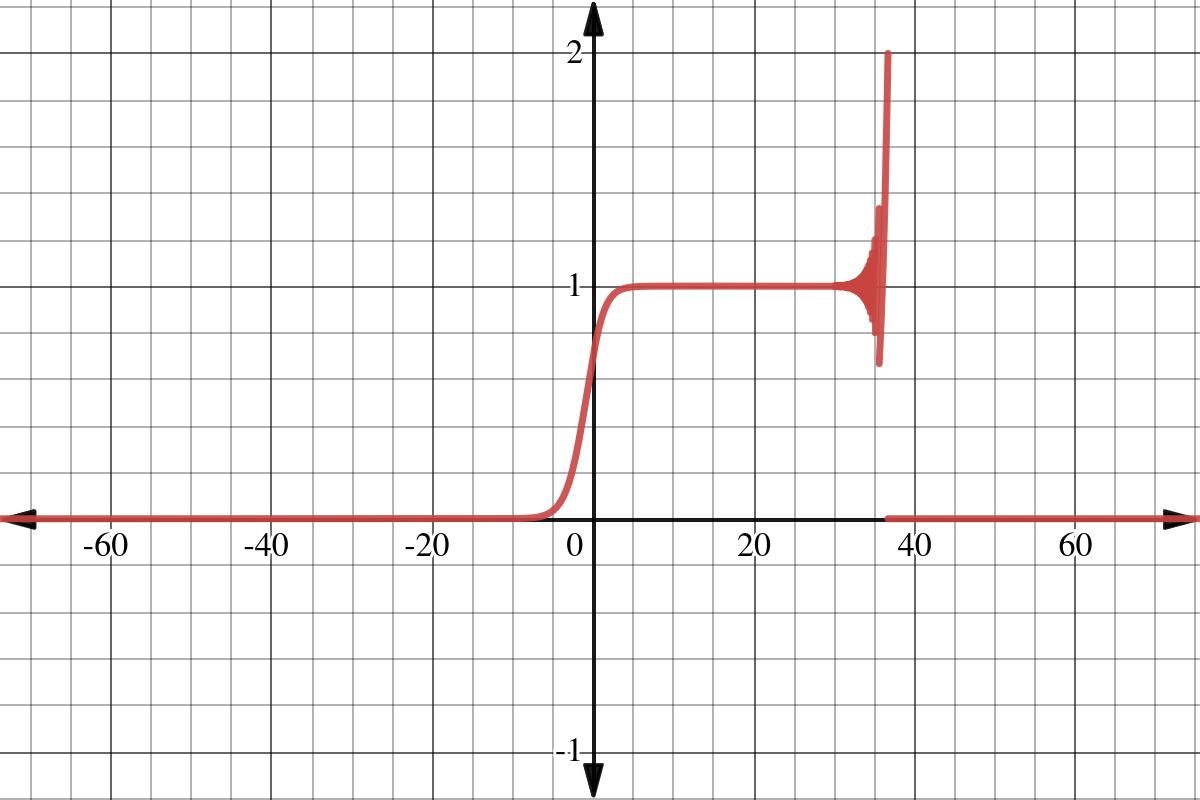
\includegraphics[width=0.62\textwidth]{../images/desmos-graph.png}
  \caption{Wykres $f(x)$ wygenerowany przy użyciu desmos.com}
\end{figure}
\begin{figure}[H]
  \centering
  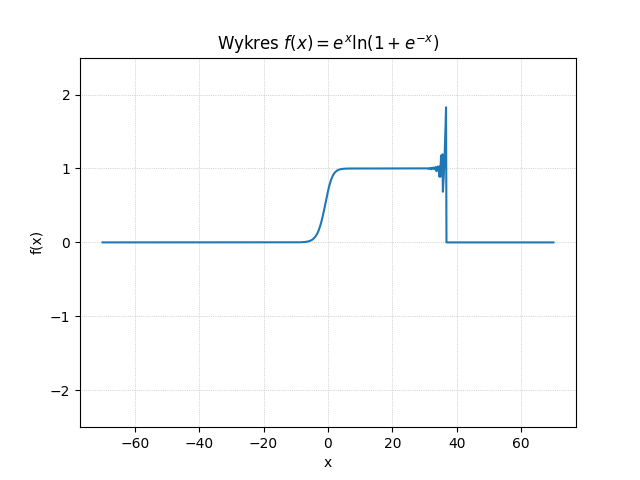
\includegraphics[width=0.8\textwidth]{../images/my-graph.png}
  \caption{Wykres $f(x)$ wygenerowany przy użyciu pythona}
\end{figure}
Na obu tych wykresach wyraźnie widać, że nie są one zgodne
z faktyczną wartością funkcji dla $x\to\infty$. Pierwsze
wahania w wartości możemy już zaobserwować od $x=27.5$,
przy $x=32$ te wahania zaczynają być już widoczne nawet
na oddalonym wykresie. W wykresie wygenerowanym przez desmos
w $x=36.736$ mamy $f(36.736) = 1.9984$ czyli błąd bezwględny
wynosi około $0.9984$. Potem oba nardędzia dają nam $f(x) = 0.0$
aż do nieskońćzoności.

\subsection*{Wyjaśnienie}
Dla coraz większych wartości $x$, $\ln{e^{-x}}$ staje się bliskie zeru,
a $e^x$ rośnie do bardzo dużych wartości. Przez to wymnażanie tych liczb skutkuje
silnym błędem. Od pewnego momentu jednak widzimy, że funkcja jest równa 0, ponieważ
$e^{-x}$ zaczyna być mniejsze od macheps, a więc dodanie
go do 1 nadal równa się 1, a $\ln{1} = 0$.





\section*{Zadanie 3}
W tym zadaniu mamy dane:
\begin{gather*}
A \in \mathbb{R}^{n \times n}\\
b = A \cdot {(1,\dots,1)}^T
\end{gather*}
Chcemy zbadać z jaką dokładnością jesteśmy w stanie
wygenerować $x$ przy pomocy:
\begin{enumerate}
  \item[a)] eliminacji Gaussa
  \item[b)] $x=A^{-1}b$
\end{enumerate}

\subsection*{Macierz Hilberta}
Za A podstawiamy macierz Hilberta stopnia n.
Macierz Hilberta to macierz dana wzorem:
\[h_{ij} = \frac{1}{i + j - 1} \quad \text{dla } i, j \in [n]\]
Wartości $x$ będę liczył dla $n \in [2,100]$,
a następnie liczył błąd względny na podstawie
normy wektorów według wzoru
$
  \frac{|x\prime - x|}{|x|}  
$.
\begin{figure}[H]
  \centering
  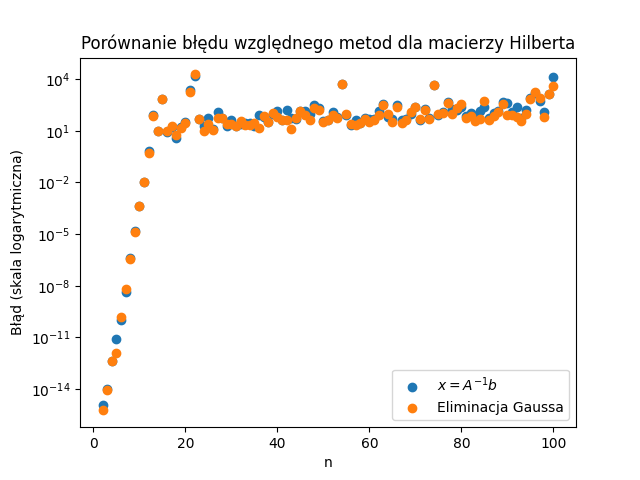
\includegraphics[width=\textwidth]{../images/hilbert.png}
  \caption{Wykres błędów dla macierzy Hilberta}
\end{figure}

\subsection*{Macierz losowa}
Tym razem za A podstawiamy macierz losową stopnia n
o wskaźniku uwarunkowania c. Konkretnie mamy:
\begin{gather*}
n \in \{5,10,20\}\\
c \in \{1,10,10^3,10^7,10^{12},10^{16}\}
\end{gather*}
Dla każdego n i c macierz losować będziemy 1000 razy
i brali z otrzymanych błędów średnią.

\begin{figure}[H]
  \centering
  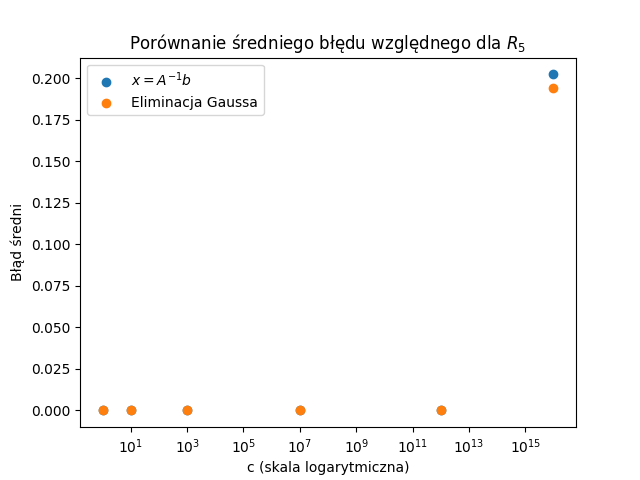
\includegraphics[width=0.8\textwidth]{../images/random_n_5.png}
  \caption{Wykres błędów dla macierzy $R_5$}
\end{figure}
\begin{figure}[H]
  \centering
  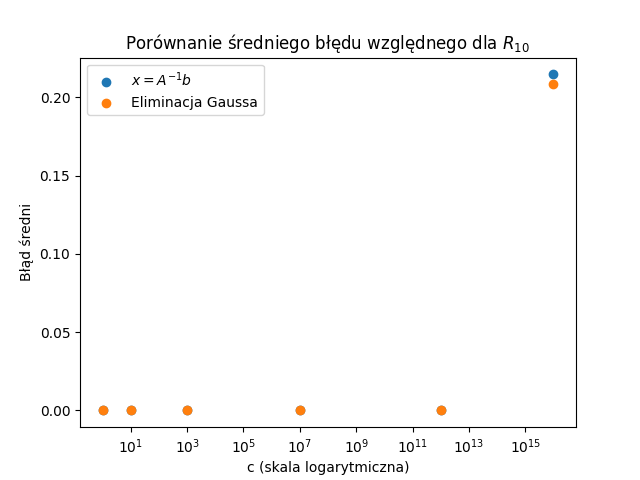
\includegraphics[width=0.8\textwidth]{../images/random_n_10.png}
  \caption{Wykres błędów dla macierzy $R_{10}$}
\end{figure}
\begin{figure}[H]
  \centering
  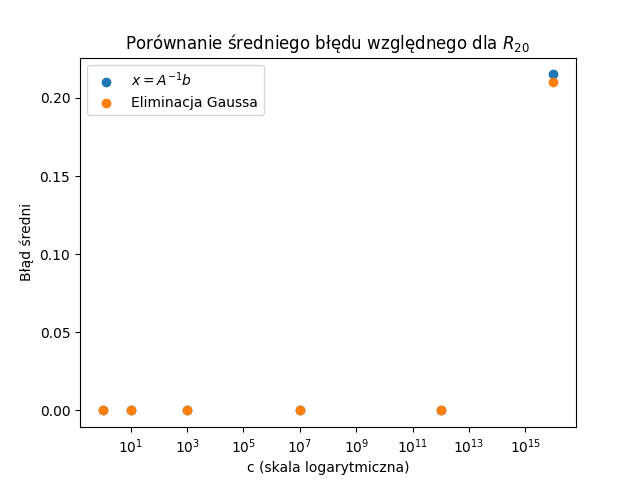
\includegraphics[width=0.8\textwidth]{../images/random_n_20.png}
  \caption{Wykres błędów dla macierzy $R_{20}$}
\end{figure}

\subsection*{Wnioski}
W przypadku obu rodzin macierzy widzimy, że obie metody
dają nam niemalże identyczne wyniki. Ponadto, błąd jest
znacznie wyższy dla macierzy Hilberta niż dla macierzy losowych.
Dzieje się tak, ponieważ precyzja Float64 jest za mała żeby
wyniki obliczeń na większych macierzach Hilberta były rzetelne.
W losowych macierzach możemy zauważyć, że dopiero dla wysokich
wartości $c$ nasz błąd zaczyna mocno odbiegać od $0$. Widzimy więc,
że przede wszystkim na podstawie wskaźniku uwarunkowania jesteśmy
w stanie określić skalę błędu.




\section*{Zadanie 4}
W tym zadaniu rozważamy wielomian Wilkinsona
$p(x) = (x - 20)(x - 19)(x - 18)(x - 17)(x - 16)
(x - 15)(x - 14)(x - 13)(x - 12)(x - 11)
(x - 10)(x - 9)(x - 8)(x - 7)(x - 6)
(x - 5)(x - 4)(x - 3)(x - 2)(x - 1)$
oraz jego postać naturalną.
Przy pomocy biblioteki Polynomials z Julii
szukamy pierwiastków $z_k$ tego wielomianu, a następnie
sprawdzamy $|p(z_k)|$, $|P(z_k)|$ i $|z_k - k|$ dla
$1 \leq k \leq 20$.
\begin{table}[h]
  \centering
  \begin{tabular}{|c|c|c|}
    \hline
    $k$ & $p(z_k)$ & $P(z_k)$ \\
    \hline
    1 & 36626.4255 & 35696.5096 \\
    2 & 181303.9337 & 176252.6003 \\
    3 & 290172.2859 & 279157.6969 \\
    4 & -2.0415e6 & -3.0271e6 \\
    5 & -2.0895e7 & -2.2917e7 \\
    6 & -1.1250e8 & -1.2902e8 \\
    7 & -4.5729e8 & -4.8051e8 \\
    8 & -1.5556e9 & -1.6380e9 \\
    9 & -4.6878e9 & -4.8771e9 \\
    10 & -1.2635e10 & -1.3639e10 \\
    11 & -3.3001e10 & -3.5856e10 \\
    12 & -7.3885e10 & -7.5333e10 \\
    13 & -1.8476e11 & -1.9606e11 \\
    14 & -3.5514e11 & -3.5751e11 \\
    15 & -8.4232e11 & -8.2163e11 \\
    16 & -1.5707e12 & -1.5515e12 \\
    17 & -3.3170e12 & -3.6947e12 \\
    18 & -6.3449e12 & -7.6501e12 \\
    19 & -1.2286e13 & -1.1435e13 \\
    20 & -2.3183e13 & -2.7924e13 \\
    \hline
  \end{tabular}
  \caption{Wartości $p(z_k)$ i $P(z_k)$ dla $k \in [1,20]$}
\end{table}
\begin{figure}[H]
  \centering
  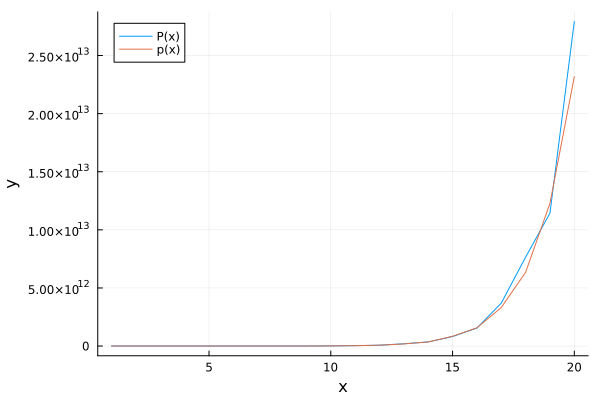
\includegraphics[width=0.8\textwidth]{../images/abs_P_vs_p.png}
  \caption{Porównanie wartości dla $P(z_k)$ i $p(z_k)$}
\end{figure}
\begin{figure}[H]
  \centering
  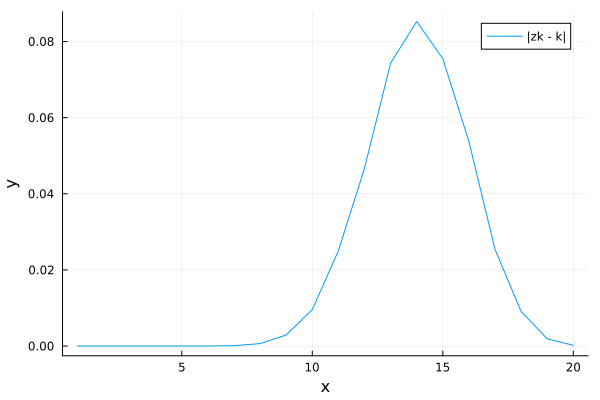
\includegraphics[width=0.8\textwidth]{../images/abs_P_roots_vs_i.png}
  \caption{$|z_k - k|$}
\end{figure}
\clearpage
\subsubsection*{Zmiana $-210$ na $-210-2^{-23}$}
\begin{table}[h]
  \centering
  \begin{tabular}{|c|c|c|}
    \hline
    $k$ & $p(z_k)$ & $P(z_k)$ \\
    \hline
    1 & $19987.8723 - 0.0i$ & $20259.8723 + 0.0i$ \\
    2 & $352369.4138 - 0.0i$ & $346541.4138 + 0.0i$ \\
    3 & $2.4162 \times 10^6 - 0.0i$ & $2.2581 \times 10^6 + 0.0i$ \\
    4 & $1.1264 \times 10^7 - 0.0i$ & $1.0543 \times 10^7 + 0.0i$ \\
    5 & $4.4757 \times 10^7 - 0.0i$ & $3.7578 \times 10^7 + 0.0i$ \\
    6 & $2.1421 \times 10^8 - 0.0i$ & $1.3141 \times 10^8 + 0.0i$ \\
    7 & $1.7846 \times 10^9 - 0.0i$ & $3.9394 \times 10^8 + 0.0i$ \\
    8 & $1.8687 \times 10^{10} - 0.0i$ & $1.1850 \times 10^9 + 0.0i$ \\
    9 & $1.3746 \times 10^{11} - 0.0i$ & $2.2255 \times 10^9 + 0.0i$ \\
    10 & $5.2761 \times 10^{11} - 1.3935 \times 10^{12}i$ & $8.8846 \times 10^9 - 5.9229 \times 10^9i$ \\
    11 & $5.2761 \times 10^{11} + 1.3935 \times 10^{12}i$ & $8.8846 \times 10^9 + 5.9229 \times 10^9i$ \\
    12 & $-2.8967 \times 10^{13} - 1.5732 \times 10^{13}i$ & $1.1009 \times 10^{10} - 2.9409 \times 10^{10}i$ \\
    13 & $-2.8967 \times 10^{13} + 1.5732 \times 10^{13}i$ & $1.1009 \times 10^{10} + 2.9409 \times 10^{10}i$ \\
    14 & $-9.2671 \times 10^{14} - 2.2906 \times 10^{14}i$ & $-6.4856 \times 10^{10} - 2.0579 \times 10^{11}i$ \\
    15 & $-9.2671 \times 10^{14} + 2.2906 \times 10^{14}i$ & $-6.4856 \times 10^{10} + 2.0579 \times 10^{11}i$ \\
    16 & $-2.7414 \times 10^{16} + 6.2826 \times 10^{14}i$ & $-4.6533 \times 10^{10} - 4.8277 \times 10^{11}i$ \\
    17 & $-2.7414 \times 10^{16} - 6.2826 \times 10^{14}i$ & $-4.6533 \times 10^{10} + 4.8277 \times 10^{11}i$ \\
    18 & $-1.3108 \times 10^{17} - 4.0454 \times 10^{17}i$ & $1.2065 \times 10^{12} - 4.3946 \times 10^{12}i$ \\
    19 & $-1.3108 \times 10^{17} + 4.0454 \times 10^{17}i$ & $1.2065 \times 10^{12} + 4.3946 \times 10^{12}i$ \\
    20 & $1.3744 \times 10^{18} + 0.0i$ & $8.7564 \times 10^{12} + 0.0i$ \\
    \hline
  \end{tabular}
  \caption{Wartości $p(z_k)$ i $P(z_k)$ dla $k \in [1,20]$ po zmianie współczynnika}
\end{table}

\begin{table}[h]
  \centering
  \begin{tabular}{|c|c|}
    \hline
    $k$ & $|z_k - k|$ \\
    \hline
    1 & 1.6431300764452317e-13\\
    2 & 5.503730804434781e-11\\
    3 & 3.3965799062229962e-9\\
    4 & 8.972436216225788e-8\\
    5 & 1.4261120897529622e-6\\
    6 & 2.0476673030955794e-5\\
    7 & 0.00039792957757978087\\
    8 & 0.007772029099445632\\
    9 & 0.0841836320674414\\
    10 & 0.6519586830380407\\
    11 & 1.1109180272716561\\
    12 & 1.665281290598479\\
    13 & 2.0458202766784277\\
    14 & 2.518835871190904\\
    15 & 2.7128805312847097\\
    16 & 2.9060018735375106\\
    17 & 2.825483521349608\\
    18 & 2.4540214463129764\\
    19 & 2.0043294443099486\\
    20 & 0.8469102151947894\\
    \hline
  \end{tabular}
  \caption{Wartości $|z_k - k|$ dla $k \in [1,20]$ po zmianie współczynnika}
\end{table}

Wyraźnie widzimy, że wyliczone wartości pierwiastków różnią się od
faktycznych wartości. Widzimy również, że nawet dla małych błędów
(rzędu e-13) mamy olbrzymie różnice w wyniku. Poza tym, nawet
pozornie nieznacząca zmiana we współczynnikach, silnie wpływa na wyniki,
do tego stopnia, że przechodzą one do ciała liczb zespolonych.
Widzimy więc, że jest to zadanie źle uwarunkowane.



\section*{Zadanie 5}
Mamy dane:
\begin{gather*}
  p_{n+1}:=p_n+rp_n(1-p_n)\\
  p_0 = 0.01\\
  r=3
\end{gather*}
\begin{figure}[H]
  \centering
  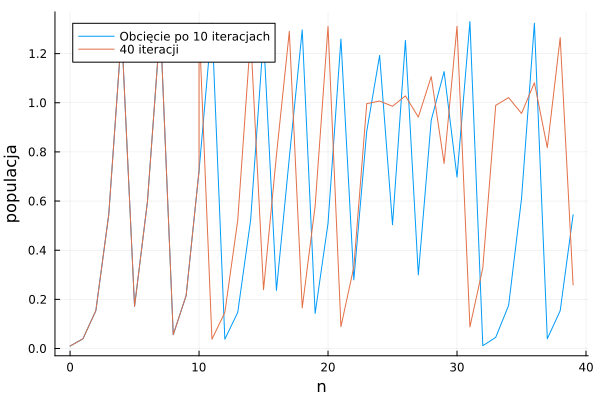
\includegraphics[width=\textwidth]{../images/ex5.png}
  \caption{Porównanie iteracji funkcji $p_n$}
\end{figure}
Jak widzimy na wykresie, do 10 iteracji obie metody są
identyczne. Natomiast po wprowadzeniu dość nieznacznej
zmiany, obcięcia do 3 miejsca po przecinku,
błąd się kumuluje tak szybko, że już po kilku iteracjach
wykresy są kompletnie niezgodne ze sobą.
\begin{figure}[H]
  \centering
  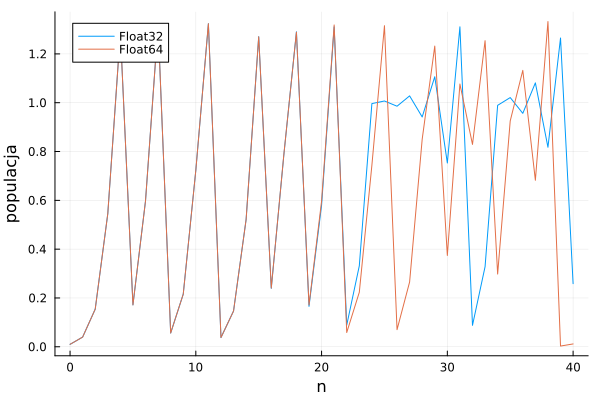
\includegraphics[width=\textwidth]{../images/ex5_f32f64.png}
  \caption{Porównanie iteracji funkcji $p_n$ dla Float32 i Float64}
\end{figure}
Przez pierwszych 10 iteracji, wyniki dla Float32 i Float64
są zgodne do 4 miejsca po przecinku. W 24 iteracji po raz pierwszy
przestają się zgadzać już na pierwszym miejscu po przecinku, a
około iteracji 27 już zupełnie nie są do siebie podobne.

Oba te eksperymenty pokazują, że symulowanie procesów
lub układów chaotycznych nie da nam żadnych rzetelnych
wyników na dłuższej przestrzeni działania symulacji
jeśli mamy do czynienia ze skończoną precyzją.
Przy różnym sprzęcie, precyzji
lub też przy małych wahaniach danych wejściowych
z czasem dostaniemy zupełnie różne wyniki, które są równie niedokładne
co takie, które wygenerowalibyśmy losowo.



\section*{Zadanie 6}
Rozważamy równanie:
\begin{gather*}
  x_{n+1}=x_n^2+c
\end{gather*}

\subsection*{Iteracja graficzna}
\begin{figure}[H]
  \centering
  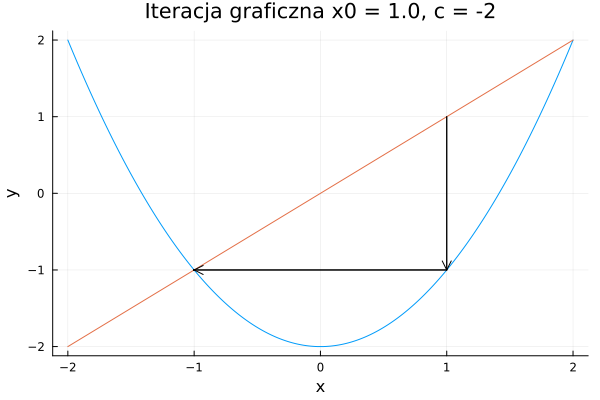
\includegraphics[width=0.8\textwidth]{../images/ex6_1.png}
  \caption{Iteracja graficzna dla $x_0=1.0$, $c=-2$}
\end{figure}
\begin{figure}[H]
  \centering
  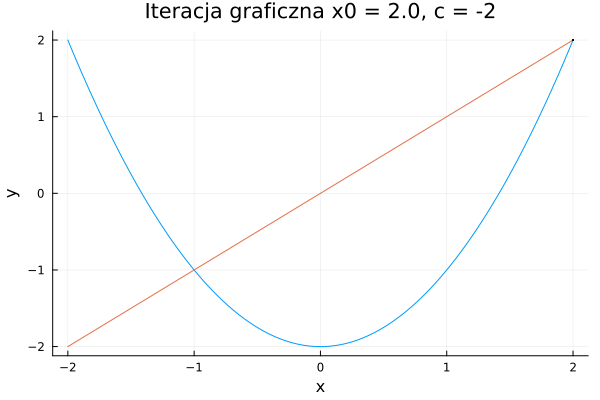
\includegraphics[width=0.8\textwidth]{../images/ex6_2.png}
  \caption{Iteracja graficzna dla $x_0=2.0$, $c=-2$}
\end{figure}
\begin{figure}[H]
  \centering
  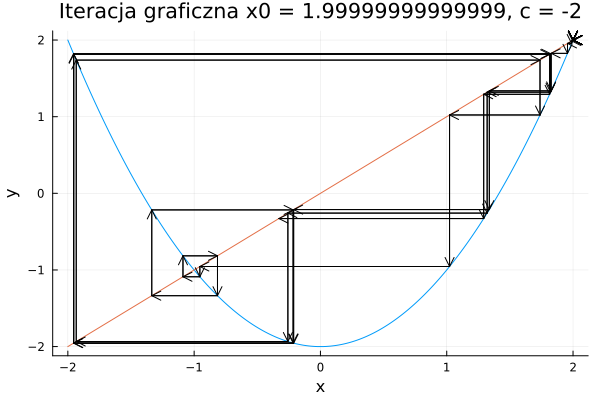
\includegraphics[width=0.8\textwidth]{../images/ex6_3.png}
  \caption{Iteracja graficzna dla $x_0=1.9999999999999$, $c=-2$}
\end{figure}
\begin{figure}[H]
  \centering
  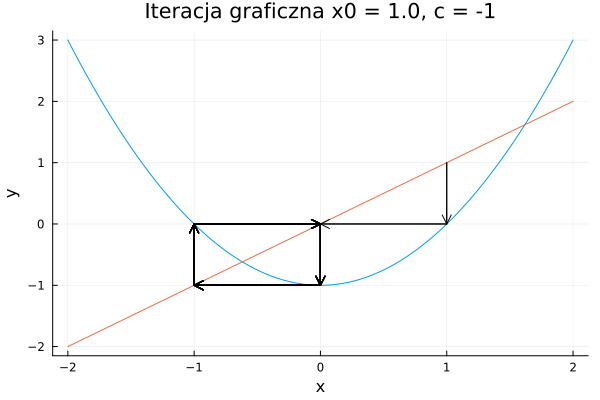
\includegraphics[width=0.8\textwidth]{../images/ex6_4.png}
  \caption{Iteracja graficzna dla $x_0=1.0$, $c=-1$}
\end{figure}
\begin{figure}[H]
  \centering
  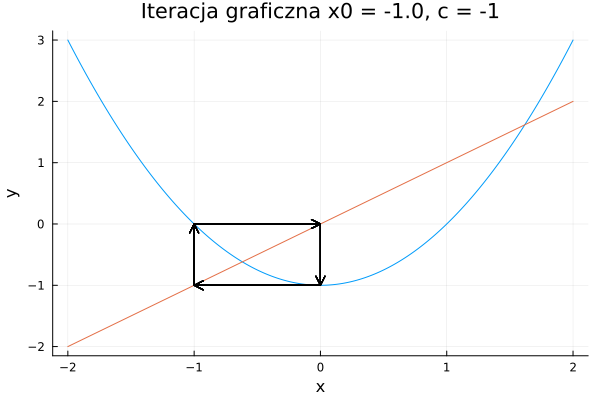
\includegraphics[width=0.8\textwidth]{../images/ex6_5.png}
  \caption{Iteracja graficzna dla $x_0=-1.0$, $c=-1$}
\end{figure}
\begin{figure}[H]
  \centering
  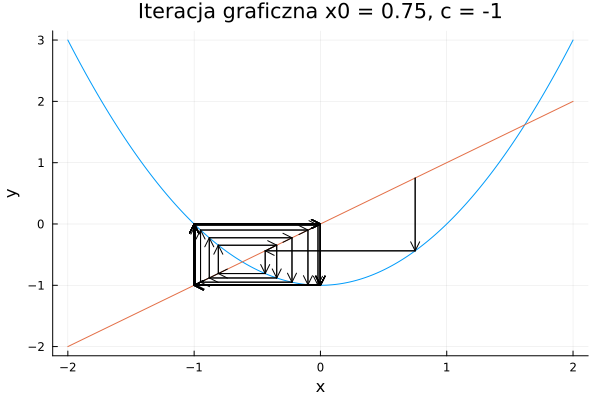
\includegraphics[width=0.8\textwidth]{../images/ex6_6.png}
  \caption{Iteracja graficzna dla $x_0=0.75$, $c=-1$}
\end{figure}
\begin{figure}[H]
  \centering
  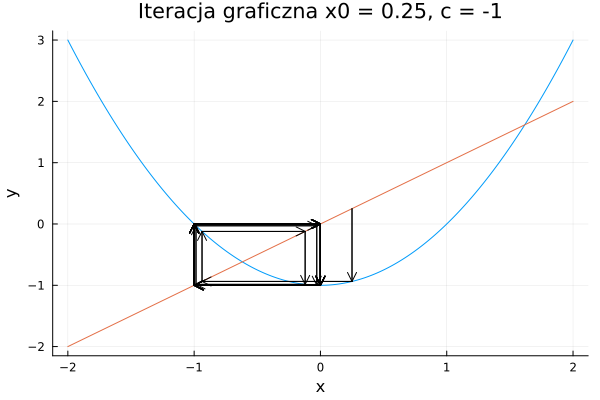
\includegraphics[width=0.8\textwidth]{../images/ex6_7.png}
  \caption{Iteracja graficzna dla $x_0=0.25$, $c=-1$}
\end{figure}

Na podstawie iteracji graficznej jesteśmy w stanie stwierdzić,
że dla danych
\begin{gather*}
  x_0=1.0,\;c=-2\\
  x_0=2.0,\;c=-2\\
  x_0=1.0,\;c=-1\\
  x_0=-1.0,\;c=-1\\
  x_0=0.75,\;c=-1\\
  x_0=0.25,\;c=-1\\
\end{gather*}
zachowanie jest stabilne, natomiast dla
\begin{gather*}
  x_0=1.9999999999999,\;c=-2\\
\end{gather*}
jest ono niestabilne.
Widzimy więc, że układ może stać się niestabilny nawet przy bardzo
niewielkich zmianach danych wejściowych.
\end{document}